\documentclass[11pt,reqno]{article}
%\input{17F-137-HomeworkTemplate}
\title{Homework \#2}
%\maketitle
%\due{Tuesday 9/12}

\headheight -10pt

%%\voffset 0.3 cm

\textheight 26cm% 25.5cm

\textwidth 18cm

\topmargin -2cm

\parindent 0pt

\oddsidemargin -1.2cm \columnsep 18pt

\usepackage{amsmath}
\usepackage{amsthm}
\usepackage{amssymb}
\usepackage{amsfonts}
\usepackage{graphicx}
\usepackage{latexsym}
\usepackage{times}
\usepackage{fancyhdr}
\usepackage{url}
\usepackage{multicol}
\usepackage{cite}
\usepackage{hyperref}
\usepackage{mathrsfs}
\usepackage[usenames]{color}
\usepackage{enumitem}
%\usepackage{verbatim}

\usepackage{subcaption}
\usepackage{setspace}


\usepackage{tikz}
\usetikzlibrary{decorations.pathreplacing}
\usetikzlibrary{positioning}
\usetikzlibrary{calc}
\usetikzlibrary{arrows,shapes,backgrounds,3d}
\usepackage{fix-cm}
\usetikzlibrary{decorations.pathreplacing,shapes,snakes}

%%
\newcommand{\coursenumber}{Math 137}
\newcommand{\coursename}{Real and Functional Analysis}


\renewcommand{\Re}[1]{\operatorname{Re} #1 }
\renewcommand{\Im}[1]{\operatorname{Im} #1}
\newcommand{\diam}{\operatorname{diam}}

%% New Commands
\newcommand{\D}{\mathbb{D}}
\newcommand{\Z}{\mathbb{Z}}
\newcommand{\R}{\mathbb{R}}
\newcommand{\Q}{\mathbb{Q}}
\newcommand{\C}{\mathbb{C}}
\newcommand{\F}{\mathbb{F}}
\newcommand{\G}{\mathcal{G}}
\newcommand{\M}{\mathcal{M}}
\newcommand{\K}{\mathbb{K}}
\newcommand{\U}{\mathcal{U}}
\newcommand{\UU}{\mathscr{U}}
\newcommand{\s}{\mathscr{S}}
\newcommand{\A}{\mathcal{A}}
\renewcommand{\L}{\mathfrak{L}}
\newcommand{\B}{\mathcal{B}}
\renewcommand{\P}{\mathcal{P}}
\newcommand{\N}{\mathbb{N}}

\DeclareMathOperator{\Aut}{Aut}



\renewcommand{\ker}{\operatorname{kernel}}
\newcommand{\ran}{\operatorname{range}}

\newcommand{\diag}{\operatorname{diag}}
\newcommand{\norm}[1]{\| #1 \|}
\newcommand{\inner}[1]{\langle #1 \rangle}
\newcommand{\E}{\mathcal{E}}
\newcommand{\V}{\mathcal{V}}
\newcommand{\W}{\mathcal{W}}
\newcommand{\WW}{\mathscr{W}}
\newcommand{\T}{\mathbb{T}}
\newcommand{\vecspan}{\operatorname{span}}
\newcommand{\interior}{\operatorname{int}}
\newcommand{\tr}{\operatorname{tr}}
\newcommand{\rank}{\operatorname{rank}}
\newcommand{\nullity}{\operatorname{nullity}}

\newcommand{\colspace}{\operatorname{colspace}}
\newcommand{\rowspace}{\operatorname{rowspace}}
\newcommand{\nullspace}{\operatorname{nullspace}}

\linespread{1}
\setlength{\parskip}{0.5ex plus 0.5ex minus 0.2ex}

%%  Matrices
\newcommand{\minimatrix}[4]{\begin{bmatrix} #1 & #2 \\ #3 & #4 \end{bmatrix}  }
\newcommand{\megamatrix}[9]{\begin{bmatrix} #1 & #2 & #3 \\ #4 & #5 & #6 \\ #7 & #8 & #9\end{bmatrix}  }

\renewcommand{\vec}[1]{{\bf #1}}
\newcommand{\ovec}{\operatorname{vec}}
\renewcommand{\labelenumi}{(\roman{enumi})}
\renewcommand{\hat}{\widehat}

\newcommand{\tworowvector}[2]{[#1\,\,#2]}
\newcommand{\threerowvector}[3]{[#1\,\,#2\,\,#3]}
\newcommand{\fourrowvector}[4]{[#1\,\,#2\,\,#3\,\,#4]}
\newcommand{\fiverowvector}[5]{[#1\,\,#2\,\,#3\,\,#4\,\,#5]}
\newcommand{\sixrowvector}[6]{[#1\,\,#2\,\,#3\,\,#4\,\,#5\,\,#6]}

\newcommand{\twovector}[2]{\begin{bmatrix} #1\\#2 \end{bmatrix} }
\newcommand{\threevector}[3]{\begin{bmatrix} #1\\#2\\#3 \end{bmatrix} }
\newcommand{\fourvector}[4]{\begin{bmatrix} #1\\#2\\#3\\#4 \end{bmatrix} }
\newcommand{\fivevector}[5]{\begin{bmatrix} #1\\#2\\#3\\#4\\#5 \end{bmatrix} }

\newcommand{\comment}[1]{\marginpar{\scriptsize\color{gray}$\bullet$\,#1}}
\newcommand{\highlight}[1]{\color{blue}#1\color{black}}

\renewcommand{\labelenumi}{\theenumi}
\renewcommand{\theenumi}{(\alph{enumi})}%
\renewcommand{\labelenumii}{\theenumii}
\renewcommand{\theenumii}{(\roman{enumii})}%
\newcommand{\due}[1]{\vspace{-0.2in}\begin{center}\textsc{due at the beginning of class \underline{#1}} \end{center}\medskip }


%%%
%%% Theorem Styles
%%%
\newtheorem{Proposition}{Proposition}
\newtheorem{Corollary}{Corollary}
\newtheorem{Theorem}{Theorem}
\newtheorem*{Thm}{Theorem}
\newtheorem{Postulate}{Postulate}
\newtheorem{Lemma}{Lemma}
\theoremstyle{definition}
\newtheorem*{Definition}{Definition}
\newtheorem*{Example}{Example}
\newtheorem*{Remark}{Remark}
\newtheorem{problem}{Exercise}
\newtheorem*{Question}{Question}

\let\oldenumerate=\enumerate
\def\enumerate{
	\oldenumerate
	\setlength{\itemsep}{1pt}
}
\let\olditemize=\itemize
\def\itemize{
	\olditemize
	\setlength{\itemsep}{5pt}
}

\allowdisplaybreaks
\pagenumbering{gobble}
\begin{document}

%\textbf{NAME:}\hrulefill
%\vspace{0.12in}

\centerline{\textbf{\Large{MATH 1512-Summer 2021-Final Exam}}}


\vspace{0.2 in}
\centerline{ \Large{July 30, 2021}}
\vspace{0.3 in}

\textbf{NAME (please print) :} \hrulefill
\vspace{0.2 in}
\begin{multicols}{2}
	\textbf{Instructor's Name:} \hrulefill \\
	\vspace{0.2 in}
	
	%\textbf{Section Number:} \hrulefill\\
	\vspace{0.2 in}
\end{multicols}
\vspace{0.2 in}

\textbf{INSTRUCTIONS:}
\begin{itemize}
	
	
	\item This is an individual exam based on what you understand.
	\item Books, notes, calculators, graphing software, etc. are not allowed
	\item You must leave your answers as exact values, such as $x=\sqrt{5}$, $t=\dfrac{\ln 3}{2}$, etc.
	\item To get full credit you must use proper mathematical notation and vocabulary, show all important steps, and present neat and organized work.  Use methods covered in this course.
	\item You will have the entire class period (1 hour and 40 minutes) for the exam.
	\item May the Force be with you!
	
	
\end{itemize}
\vspace{0.08 in}


\newpage
	
	\begin{enumerate}
		\item[1.]  (15 pts) 
		\begin{enumerate}
			
			\item State the mathematical definition of the derivative $f'(x)$ of a function $f(x)$ as a limit.
			
			\vspace{1.5in}
			
			\item Use the limit definition to find the derivative of $f(x)=\frac{2}{\sqrt{2x+3}}$. You must use the limit definition to receive any credit.
			
		\end{enumerate}
		\newpage
		\item[2.](15 pts) Find the derivatives of the following functions
		\begin{enumerate}
			%\item $y = [(2x + 1)^{-1} + 3]^{-1}$
			%\vspace{5 cm}
			\item $f(x) = \frac{\sin^3 x}{e^{x^2}}$ 
			\vspace{10cm}
			\item $g(x) = \sqrt[4]{x^3 - 4x^2 + 2}$
		\end{enumerate}
		\newpage
		\item[3.](25 pts) Evaluate the following integrals
			\begin{enumerate}
				\item $\int \frac{2}{x\sqrt{x}} \; dx$ 
			%	\vspace{4cm}
				%\item $\int \frac{x^2}{\sqrt[3]{1 - x^3}} \; dx$
				\vspace{6cm}
				\item $\int_{0}^{\sqrt{\pi}/2} x \sec^2 (x^2) \tan(x^2) \;dx$
			\end{enumerate}
		\newpage
		\item[4.] (20 pts)The error function (denoted as erf) is defined as $$\textnormal{erf }x = \frac{2}{\sqrt{\pi}} \int_{0}^{x} e^{-t^2} \; dt.$$ 
		\begin{enumerate}
			\item Find the first and second derivatives of the error function.
			\vspace{5cm}
			\item The error function has two horizontal asymptotes - $\lim_{x \to \infty} \textnormal{erf } x = 1$ and $\lim_{x \to -\infty} \textnormal{erf } x = -1$. Using this and the first and second derivatives from the previous part, sketch a graph of the error function labeling the points of inflection and local extrema if any exist.
		\end{enumerate}
		\newpage
		\item[5.] (15 pts) Find the area between $y = \cos\left(\frac{\pi x}{2}\right)$ and $y = 1 - x^2$ in the first quadrant. 
		\newpage
		\item[6.] (25 pts) Let $S$ be the region of the $xy$-plane bounded above by the curve $x^3y = 64$, below by the line $y = 1$, on the left by the line $x = 2$ and on the right by the line $x = 4$. Find the volume of the solid when rotating $S$ around the line $x = 2$. 
		\newpage
		\item[7.] (10 pts) Find the arc length of $y = e^{x/2} + e^{-x/2}$ on the interval $[0, 1]$. 
		\newpage
		\textbf{DIRECTIONS:} Pick \textbf{ONE} problem from Problems 8-10 to complete. Make sure it is clear which problem you have chosen and which ones you have not chosen. 
		\item[8.] (25 pts) You want to see a certain number $n$ of items in order to maximize your profit. Market research tells you that if you set the price at \$1.50, you will be able to sell $5000$ items and for every 10 cents you lower the price below \$1.50 you will be able to sell another 1000 items. Suppose that your fixed costs total \$2000, and the per item cost of production is \$0.50. Find the price to set per item and number of items sold in order to maximize profit. Recall that profit = revenue - cost and revenue = number of items sold times price per item.
		\newpage
		\item[9.] (25 pts) Much like how we found volume of a solid of revolution using the sum of circular cross sections, we can also find the surface area of solid of revolution using the slice and sum method where we slice up a surface and sum the surface areas of the frustum of cones. The result we get is that if the area under $f(x)$ on the interval $[a, b]$ is rotated about the $x$-axis, the surface area of the solid of revolution is given by the integral 
		$$ SA = \int_{a}^{b} 2\pi f(x) \sqrt{1 + [f'(x)]^2} \; dx.$$
		
		Recall that we can create a sphere of radius $r$ by rotating $y = \sqrt{r^2 - x^2}$ about the $x$-axis on the interval $[-r, r]$. Using the formula above, show that the surface area of a sphere of radius $r$ is $4 \pi r^2$. 
		\newpage
		\item[10.] (25 pts) A swing consists of a board at the end of a 10 ft long rope. Think of the board as a point $P$ at the end of the rope and let $Q$ be the point of attachment at the other end. Suppose that the swing is directly below $Q$ at time $t = 0$ and is being pushed by someone who walks at 6 ft/sec from left to right. Find how fast the swing is rising after 1 sec. (Hint: Use the picture given) 
		
		\begin{figure}[h!]
			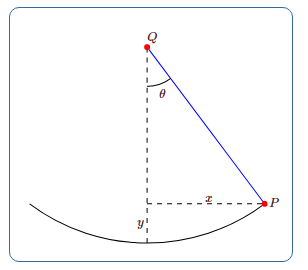
\includegraphics[scale=0.8]{Capture.PNG}
		\end{figure}
		
	
	\end{enumerate}
	
	
\end{document}
